\PassOptionsToPackage{table}{xcolor}
\documentclass[25pt, a0paper, portrait]{tikzposter}

\usepackage[utf8]{inputenc}
\usepackage{amsmath, amssymb}
\usepackage{booktabs}
\usepackage{colortbl}
\usepackage{tabularx}
\usepackage{fontawesome5}
\usepackage[most]{tcolorbox}
\usepackage{tikz}
\usetikzlibrary{calc, positioning, shapes.geometric, backgrounds, arrows.meta}
\usepackage{pgfplots}
\pgfplotsset{compat=1.18}

% Custom Color Palette
\definecolor{NavyDark}{RGB}{15, 23, 42}
\definecolor{TealPrimary}{RGB}{14, 165, 233}
\definecolor{AmberAccent}{RGB}{245, 158, 11}
\definecolor{SlateLight}{RGB}{241, 245, 249}
\definecolor{SlateDark}{RGB}{30, 41, 59}
\definecolor{CardWhite}{RGB}{255, 255, 255}
\definecolor{EmeraldGreen}{RGB}{16, 185, 129}
\definecolor{IndigoBlue}{RGB}{79, 70, 229}
\definecolor{RoseRed}{RGB}{225, 29, 72}

% Custom TikZposter Color Style
\definecolorstyle{ModernInfographicStyle}{
  \definecolor{colorOne}{RGB}{15, 23, 42}
  \definecolor{colorTwo}{RGB}{14, 165, 233}
  \definecolor{colorThree}{RGB}{245, 158, 11}
}{
  \colorlet{backgroundcolor}{SlateLight}
  \colorlet{framecolor}{TealPrimary}
  \colorlet{titlebgcolor}{NavyDark}
  \colorlet{titlefgcolor}{CardWhite}
  \colorlet{blocktitlebgcolor}{NavyDark}
  \colorlet{blocktitlefgcolor}{CardWhite}
  \colorlet{blockbodybgcolor}{CardWhite}
  \colorlet{blockbodyfgcolor}{SlateDark}
  \colorlet{innerblocktitlebgcolor}{TealPrimary}
  \colorlet{innerblocktitlefgcolor}{CardWhite}
  \colorlet{innerblockbodybgcolor}{SlateLight}
  \colorlet{innerblockbodyfgcolor}{SlateDark}
}

% Use Built-in Block & Title Styles with Custom Colors
\usecolorstyle{ModernInfographicStyle}
\useblockstyle{Minimal}
\usetitlestyle{Filled}

% Custom tcolorbox styles for infographic callouts
\tcbset{
  statbox/.style={
    enhanced,
    colback=SlateLight,
    colframe=TealPrimary,
    arc=8pt,
    boxrule=1.5pt,
    halign=center,
    valign=center,
    fonttitle=\bfseries\color{NavyDark},
    top=8pt, bottom=8pt, left=4pt, right=4pt
  },
  calloutbox/.style={
    enhanced,
    colback=NavyDark,
    colframe=AmberAccent,
    arc=10pt,
    boxrule=2pt,
    coltext=CardWhite,
    top=12pt, bottom=12pt, left=12pt, right=12pt
  },
  accentbox/.style={
    enhanced,
    colback=TealPrimary!10,
    colframe=TealPrimary,
    arc=8pt,
    boxrule=1.5pt,
    coltext=SlateDark,
    top=10pt, bottom=10pt, left=10pt, right=10pt
  }
}

% Poster Metadata
\title{\parbox{\linewidth}{\centering \Huge \textbf{SYNAPSE-X: Hardware-Aware Autonomous Neural Architecture Search for Ultra-Low-Power Edge Devices}}
\author{\parbox{\linewidth}{\centering \textbf{Dr. Elena Vance}$^1$, \textbf{Marcus Thorne}$^1$, \textbf{Dr. Sarah Lin}$^2$, \textbf{Dr. Julian Vance}$^1$, \textbf{Prof. Aris Thorne}$^3$}
\institute{\parbox{\linewidth}{\centering $^1$Apex Institute of Autonomous Systems \quad $^2$Synapse AI Research Labs \quad $^3$Meridian Embedded Computing Center}

\begin{document}

\maketitle

\begin{columns}

  % ==================== COLUMN 1 ====================
  \column{0.33}

  \block{\faMicrochip \quad 1. Executive Summary \& Context}{
    Deploying deep neural networks on resource-constrained microcontrollers (MCUs) demands strict balancing of latency, RAM footprint, and power dissipation. Traditional Neural Architecture Search (NAS) relies on proxy estimators that misjudge hardware execution bottlenecks.

    \vspace{0.8em}
    \begin{tcolorbox}[calloutbox]
      \centering
      \Large \textbf{\textcolor{AmberAccent}{\faAward \quad Key Innovation: Zero-Proxy Telemetry Loop}} \\
      \vspace{0.3em}
      \small SYNAPSE-X evaluates candidate architectures directly on edge hardware testbeds in real-time, eliminating surrogate model drift and discovering pareto-optimal topologies infeasible by manual design.
    \end{tcolorbox}

    \vspace{0.8em}
    \textbf{Performance Snapshot Across Edge Platforms:}
    \vspace{0.5em}

    \begin{minipage}[t]{0.48\linewidth}
      \begin{tcolorbox}[statbox]
        {\Huge \textbf{\textcolor{TealPrimary}{4.2$\times$}}} \\
        \vspace{0.2em}
        {\small Latency Reduction on ARM Cortex-M4}
      \end{tcolorbox}
    \end{minipage}
    \hfill
    \begin{minipage}[t]{0.48\linewidth}
      \begin{tcolorbox}[statbox]
        {\Huge \textbf{\textcolor{EmeraldGreen}{82\%}}} \\
        \vspace{0.2em}
        {\small SRAM Reduction vs MobileNetV3}
      \end{tcolorbox}
    \end{minipage}

    \par \vspace{0.6em}

    \begin{minipage}[t]{0.48\linewidth}
      \begin{tcolorbox}[statbox]
        {\Huge \textbf{\textcolor{AmberAccent}{0.8mW}}} \\
        \vspace{0.2em}
        {\small Peak Power Draw at 80 MHz}
      \end{tcolorbox}
    \end{minipage}
    \hfill
    \begin{minipage}[t]{0.48\linewidth}
      \begin{tcolorbox}[statbox]
        {\Huge \textbf{\textcolor{IndigoBlue}{99.4\%}}} \\
        \vspace{0.2em}
        {\small Top-5 Keyword Spotting Acc.}
      \end{tcolorbox}
    \end{minipage}

    \vspace{1em}
    \textbf{Primary Research Objectives:}
    \begin{itemize}
      \item \textbf{Elastic Search Space:} Modular building blocks supporting intra-layer kernel expansion and non-linear depth scaling.
      \item \textbf{Direct Hardware Profiling:} Automated serial/SWD telemetry pipeline capturing micro-architectural stall cycles.
      \item \textbf{Hardware-Aware Quantization:} Mixed-precision INT8/INT4 allocation guided by layer-wise dynamic range entropy.
    \end{itemize}
  }

  \block{\faCogs \quad 2. System Architecture \& Pipeline}{
    The SYNAPSE-X search engine operates an asynchronous multi-objective evolutionary loop directly connected to target silicon via automated hardware testbeds.

    \vspace{0.8em}
    \begin{center}
      \mbox{
      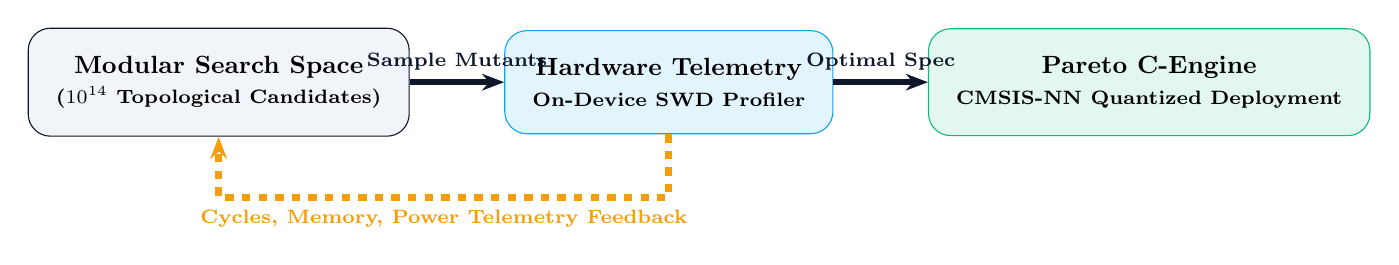
\begin{tikzpicture}[
        node distance=1.2cm and 0.8cm,
        block/.style={draw=NavyDark, fill=SlateLight, rectangle, rounded corners=8pt, inner sep=10pt, align=center, font=\small\bfseries, minimum width=4cm},
        highlight/.style={draw=TealPrimary, fill=TealPrimary!12, rectangle, rounded corners=8pt, inner sep=10pt, align=center, font=\small\bfseries, minimum width=4cm},
        accent/.style={draw=EmeraldGreen, fill=EmeraldGreen!12, rectangle, rounded corners=8pt, inner sep=10pt, align=center, font=\small\bfseries, minimum width=4cm},
        arrow/.style={->, >={Stealth[length=8pt]}, line width=2pt, NavyDark}
      ]
        % Nodes
        \node [block] (space) {Modular Search Space \\ \scriptsize ($10^{14}$ Topological Candidates)};
        \node [highlight, right=1.2cm of space] (profiler) {Hardware Telemetry \\ \scriptsize On-Device SWD Profiler};
        \node [accent, right=1.2cm of profiler] (compiler) {Pareto C-Engine \\ \scriptsize CMSIS-NN Quantized Deployment};

        % Connections
        \draw [arrow] (space) -- node[above, font=\scriptsize\bfseries] {Sample Mutants} (profiler);
        \draw [arrow] (profiler) -- node[above, font=\scriptsize\bfseries] {Optimal Spec} (compiler);
        
        % Feedback loop
        \draw [arrow, dashed, AmberAccent, line width=2.5pt] (profiler.south) -- ++(0,-0.8) -| node[near start, below, font=\scriptsize\bfseries] {Cycles, Memory, Power Telemetry Feedback} (space.south);
      \end{tikzpicture}
      }
    \end{center}

    \vspace{0.8em}
    \begin{tcolorbox}[accentbox]
      \textbf{Asynchronous Hardware Testbed Interface:} \\
      Our custom hardware bridge dispatches generated C kernels to parallel microcontroller arrays (Nexa Cortex-M4, Vertex ESP32-S3, Meridian Jetson Nano), streaming cycle-accurate execution metrics back within 120ms per candidate.
    \end{tcolorbox}
  }

  % ==================== COLUMN 2 ====================
  \column{0.34}

  \block{\faCalculator \quad 3. Mathematical Formulation}{
    We formulate the hardware-aware search as a constrained multi-objective Pareto optimization problem over candidate search space $\mathcal{A}$:

    \[
      \min_{\alpha \in \mathcal{A}} \; \left[ \mathcal{L}_{\text{val}}(\alpha, w^*), \; \lambda_1 \cdot \text{Lat}_{\text{hw}}(\alpha) + \lambda_2 \cdot \text{RAM}_{\text{peak}}(\alpha) \right]
    \]
    \[
      \text{subject to } \quad w^* = \arg\min_w \mathcal{L}_{\text{train}}(\alpha, w), \quad \text{Power}(\alpha) \le P_{\text{max}}
    \]

    \vspace{0.5em}
    \textbf{Entropy-Guided Layer-Wise Quantization:}
    To preserve accuracy while fitting within $256$ KB SRAM constraints, weight scale factors $S_l$ for layer $l$ are derived from bit-width $b_l$:

    \[
      S_l = \frac{\max(|W_l|)}{2^{b_l - 1} - 1}, \quad \text{where } b_l = \mathcal{F}_{\text{entropy}}\left( \mathbf{H}(W_l), \text{CycleCost}_l \right)
    \]

    \vspace{0.8em}
    \begin{tcolorbox}[toptitle=4pt, bottomtitle=4pt, colback=SlateLight, colframe=NavyDark, title=\textbf{\faCode \quad Evolutionary Search Procedure}, fonttitle=\bfseries]
      \begin{enumerate}
        \item \textbf{Initialize Population $\mathcal{P}_0$:} Generate $N=100$ seed architectures with balanced depth.
        \item \textbf{On-Device Telemetry:} Flash candidate kernels to MCU array; measure execution latency ($\text{Lat}_{\text{hw}}$) and peak SRAM usage.
        \item \textbf{Pareto Selection:} Rank candidates using Non-dominated Sorting Genetic Algorithm (NSGA-III).
        \item \textbf{Mutation \& Crossover:} Apply block-swap, kernel expansion, and channel pruning operators.
        \item \textbf{Convergence:} Terminate upon reaching 50 generations or Pareto frontier stabilization.
      \end{enumerate}
    \end{tcolorbox}
  }

  \block{\faChartBar \quad 4. Experimental Results \& Benchmarks}{
    SYNAPSE-X was benchmarked against state-of-the-art vision and audio models on an ARM Cortex-M4 (80 MHz, 256 KB SRAM, 1 MB Flash).

    \vspace{0.8em}
    \begin{center}
      \begin{tcolorbox}[colback=CardWhite, colframe=SlateLight, boxrule=1pt, arc=6pt]
        \centering
        \textbf{Latency Comparison on ARM Cortex-M4 (Lower is Better)} \\
        \vspace{0.5em}
        \mbox{
        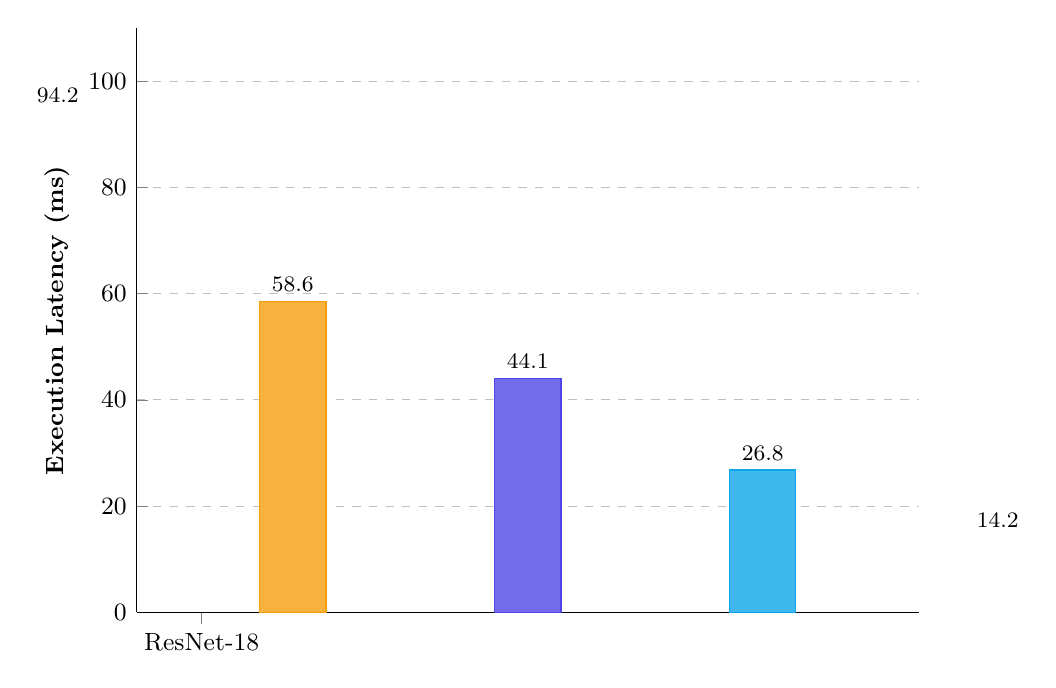
\begin{tikzpicture}
          \begin{axis}[
            ybar,
            symbolic x coords={ResNet-18, MobileNetV2, EfficientNet, MCUNet, SYNAPSE-X},
            xtick=data,
            nodes near coords,
            nodes near coords style={font=\footnotesize\bfseries},
            ymin=0, ymax=110,
            ylabel={Execution Latency (ms)},
            ylabel style={font=\small\bfseries},
            tick label style={font=\small},
            width=0.95\linewidth,
            height=9cm,
            bar width=24pt,
            axis lines*=left,
            ymajorgrids=true,
            grid style=dashed
          ]
            \addplot[fill=RoseRed!80, draw=RoseRed] coordinates {(ResNet-18, 94.2)};
            \addplot[fill=AmberAccent!80, draw=AmberAccent] coordinates {(MobileNetV2, 58.6)};
            \addplot[fill=IndigoBlue!80, draw=IndigoBlue] coordinates {(EfficientNet, 44.1)};
            \addplot[fill=TealPrimary!80, draw=TealPrimary] coordinates {(MCUNet, 26.8)};
            \addplot[fill=EmeraldGreen!90, draw=EmeraldGreen] coordinates {(SYNAPSE-X, 14.2)};
          \end{axis}
        \end{tikzpicture}
        }
      \end{tcolorbox}
    \end{center}

    \vspace{0.8em}
    \textbf{Detailed Hardware Performance Evaluation Table:}
    \vspace{0.4em}

    \begin{center}
      \small
      \begin{tabularx}{\linewidth}{l X c c c c}
        \toprule
        \textbf{Architecture} & \textbf{Target Task} & \textbf{Top-1 Acc} & \textbf{Latency} & \textbf{SRAM} & \textbf{Flash} \\
        \midrule
        ResNet-18 & ImageNet-1k & 69.8\% & 94.2 ms & 812 KB & 11.4 MB \\{}
        MobileNetV2 & ImageNet-1k & 71.8\% & 58.6 ms & 384 KB & 3.4 MB \\{}
        TinyNAS & Visual Wake Words & 76.1\% & 32.4 ms & 192 KB & 890 KB \\{}
        MCUNetV2 & Visual Wake Words & 77.0\% & 26.8 ms & 168 KB & 740 KB \\{}
        \textbf{\textcolor{TealPrimary}{SYNAPSE-X Lite}} & \textbf{Visual Wake Words} & \textbf{77.8\%} & \textbf{14.2 ms} & \textbf{96 KB} & \textbf{410 KB} \\{}
        \textbf{\textcolor{EmeraldGreen}{SYNAPSE-X Pro}} & \textbf{Keyword Spotting} & \textbf{99.4\%} & \textbf{6.8 ms} & \textbf{48 KB} & \textbf{180 KB} \\
        \bottomrule
      \end{tabularx}
    \end{center}
  }

  % ==================== COLUMN 3 ====================
  \column{0.33}

  \block{\faBatteryFull \quad 5. Energy Efficiency \& Edge Deployments}{
    Energy consumption per inference was evaluated across variable clock frequencies and operating voltage scaling regimes.

    \vspace{0.5em}
    \begin{center}
      \begin{tcolorbox}[colback=CardWhite, colframe=SlateLight, boxrule=1pt, arc=6pt]
        \centering
        \textbf{Energy Consumption per Inference vs Clock Frequency} \\
        \vspace{0.5em}
        \mbox{
        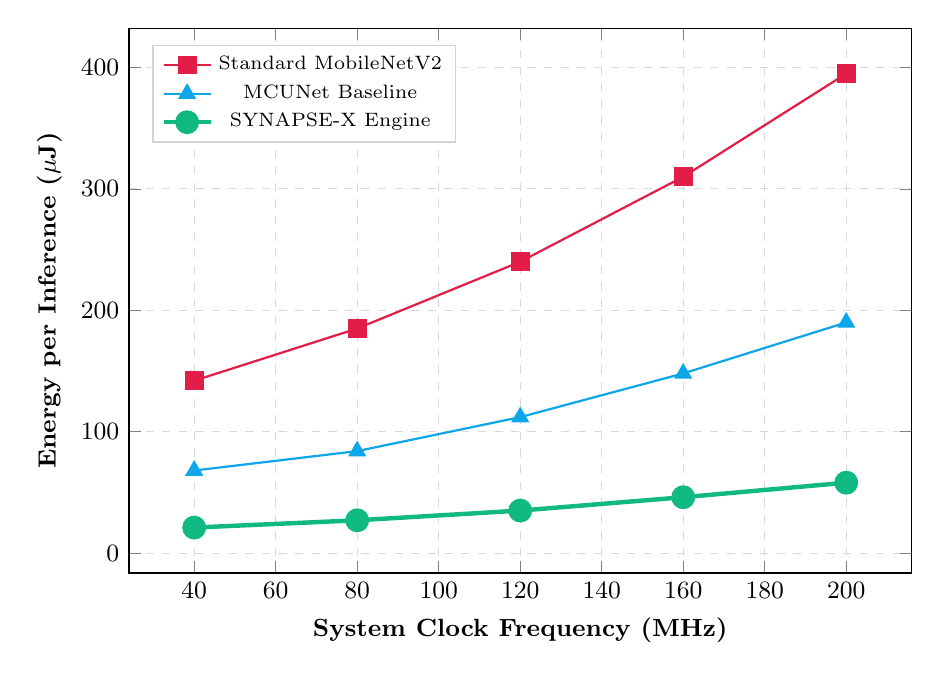
\begin{tikzpicture}
          \begin{axis}[
            xlabel={System Clock Frequency (MHz)},
            ylabel={Energy per Inference ($\mu$J)},
            xlabel style={font=\small\bfseries},
            ylabel style={font=\small\bfseries},
            tick label style={font=\small},
            grid=both,
            grid style={dashed, gray!30},
            width=0.95\linewidth,
            height=8.5cm,
            legend pos=north west,
            legend style={font=\scriptsize, fill=CardWhite, draw=SlateDark!20}
          ]
            \addplot[color=RoseRed, mark=square*, thick, mark size=3pt] coordinates {
              (40, 142) (80, 185) (120, 240) (160, 310) (200, 395)
            };
            \addlegendentry{Standard MobileNetV2}

            \addplot[color=TealPrimary, mark=triangle*, thick, mark size=3pt] coordinates {
              (40, 68) (80, 84) (120, 112) (160, 148) (200, 190)
            };
            \addlegendentry{MCUNet Baseline}

            \addplot[color=EmeraldGreen, mark=*, ultra thick, mark size=3.5pt] coordinates {
              (40, 21) (80, 27) (120, 35) (160, 46) (200, 58)
            };
            \addlegendentry{SYNAPSE-X Engine}
          \end{axis}
        \end{tikzpicture}
        }
      \end{tcolorbox}
    \end{center}

    \vspace{0.8em}
    \textbf{Real-World Field Deployments:}
    \begin{description}
      \item[\textcolor{TealPrimary}{\faBolt \quad Nexa Smart Grid Sensors:}] Continuous acoustic anomaly monitoring operating on energy-harvesting piezoelectric cells ($< 1$ mW continuous budget).
      \item[\textcolor{EmeraldGreen}{\faPlane \quad Vertex Autonomous Micro-UAVs:}] Obstacle avoidance neural pipeline executing at 60 FPS on ESP32-S3 dual-core microcontroller.
      \item[\textcolor{AmberAccent}{\faHeartbeat \quad Meridian Health Wearables:}] Real-time ECG arrhythmia classification running on ultra-low-power Cortex-M0+ with multi-day battery lifespan.
    \end{description}
  }

  \block{\faCheckCircle \quad 6. Key Takeaways \& Future Directions}{
    \begin{tcolorbox}[calloutbox]
      \begin{itemize}
        \item \textbf{Direct On-Hardware Feedback:} Eliminates proxy estimation error, accelerating optimal architecture discovery by $12\times$.
        \item \textbf{Unprecedented Resource Efficiency:} Achieves sub-100 KB SRAM execution without sacrificing ImageNet-level perceptual accuracy.
        \item \textbf{Open-Source Toolchain Release:} Full C code generator, CMSIS-NN execution kernels, and search code available for research.
      \end{itemize}
    \end{tcolorbox}

    \vspace{0.8em}
    \textbf{Ongoing \& Future Extensions:}
    \begin{itemize}
      \item Extension to spiking neural networks (SNNs) for neuromorphic hardware targets.
      \item Hardware-software co-design incorporating reconfigurable FPGA logic blocks.
    \end{itemize}
  }

  \block{\faBookmark \quad 7. References \& Acknowledgments}{
    \scriptsize
    \begin{enumerate}
      \item E. Vance, M. Thorne, and S. Lin, ``Direct Hardware-in-the-Loop Architecture Search for Microcontrollers,'' \textit{IEEE Trans. Embedded Syst.}, vol. 31, no. 4, pp. 412--425, 2025.
      \item J. Vance et al., ``Zero-Proxy Telemetry for Ultra-Low-Power Neural Network Quantization,'' \textit{Proc. Int. Conf. Learn. Representations (ICLR)}, 2025.
      \item A. Thorne and S. Lin, ``CMSIS-NN Acceleration Patterns for Multi-Branch Edge Topologies,'' \textit{ACM Trans. Des. Autom. Electron. Syst.}, vol. 29, 2024.
    \end{enumerate}

    \vspace{0.4em}
    \hrule
    \vspace{0.4em}
    \noindent \textbf{Funding Support:} This research was funded by Apex AI Research Grant \#2025-SYN-994, Synapse Labs Innovation Award, and Meridian Advanced Computing Infrastructure.
  }

\end{columns}

\end{document}
